\documentclass[12pt,a4paper]{article}


\usepackage[utf8]{vietnam}
\usepackage[vietnamese]{babel} 

\usepackage[left=1.5cm, right=1.5cm, top=1.5cm, bottom=1.5cm]{geometry}

\usepackage{graphicx} 
\usepackage{xcolor} 
\usepackage{enumitem} 
\usepackage{hyperref} 
\usepackage{titlesec} 

\setlist[itemize]{
    leftmargin=1.5em, 
    label={\scalebox{0.7}{\textbullet}},
    noitemsep, 
    topsep=0pt, 
    parsep=0pt
}


\definecolor{primary}{HTML}{8F8F8F} 
\urlstyle{same}


\titleformat{\section}{\large\bfseries\color{primary}\uppercase}{}{0em}{}[\titlerule]
\titlespacing*{\section}{0pt}{12pt}{8pt}

\begin{document}


\noindent

\begin{minipage}[b]{0.25\textwidth}
    \raggedright
    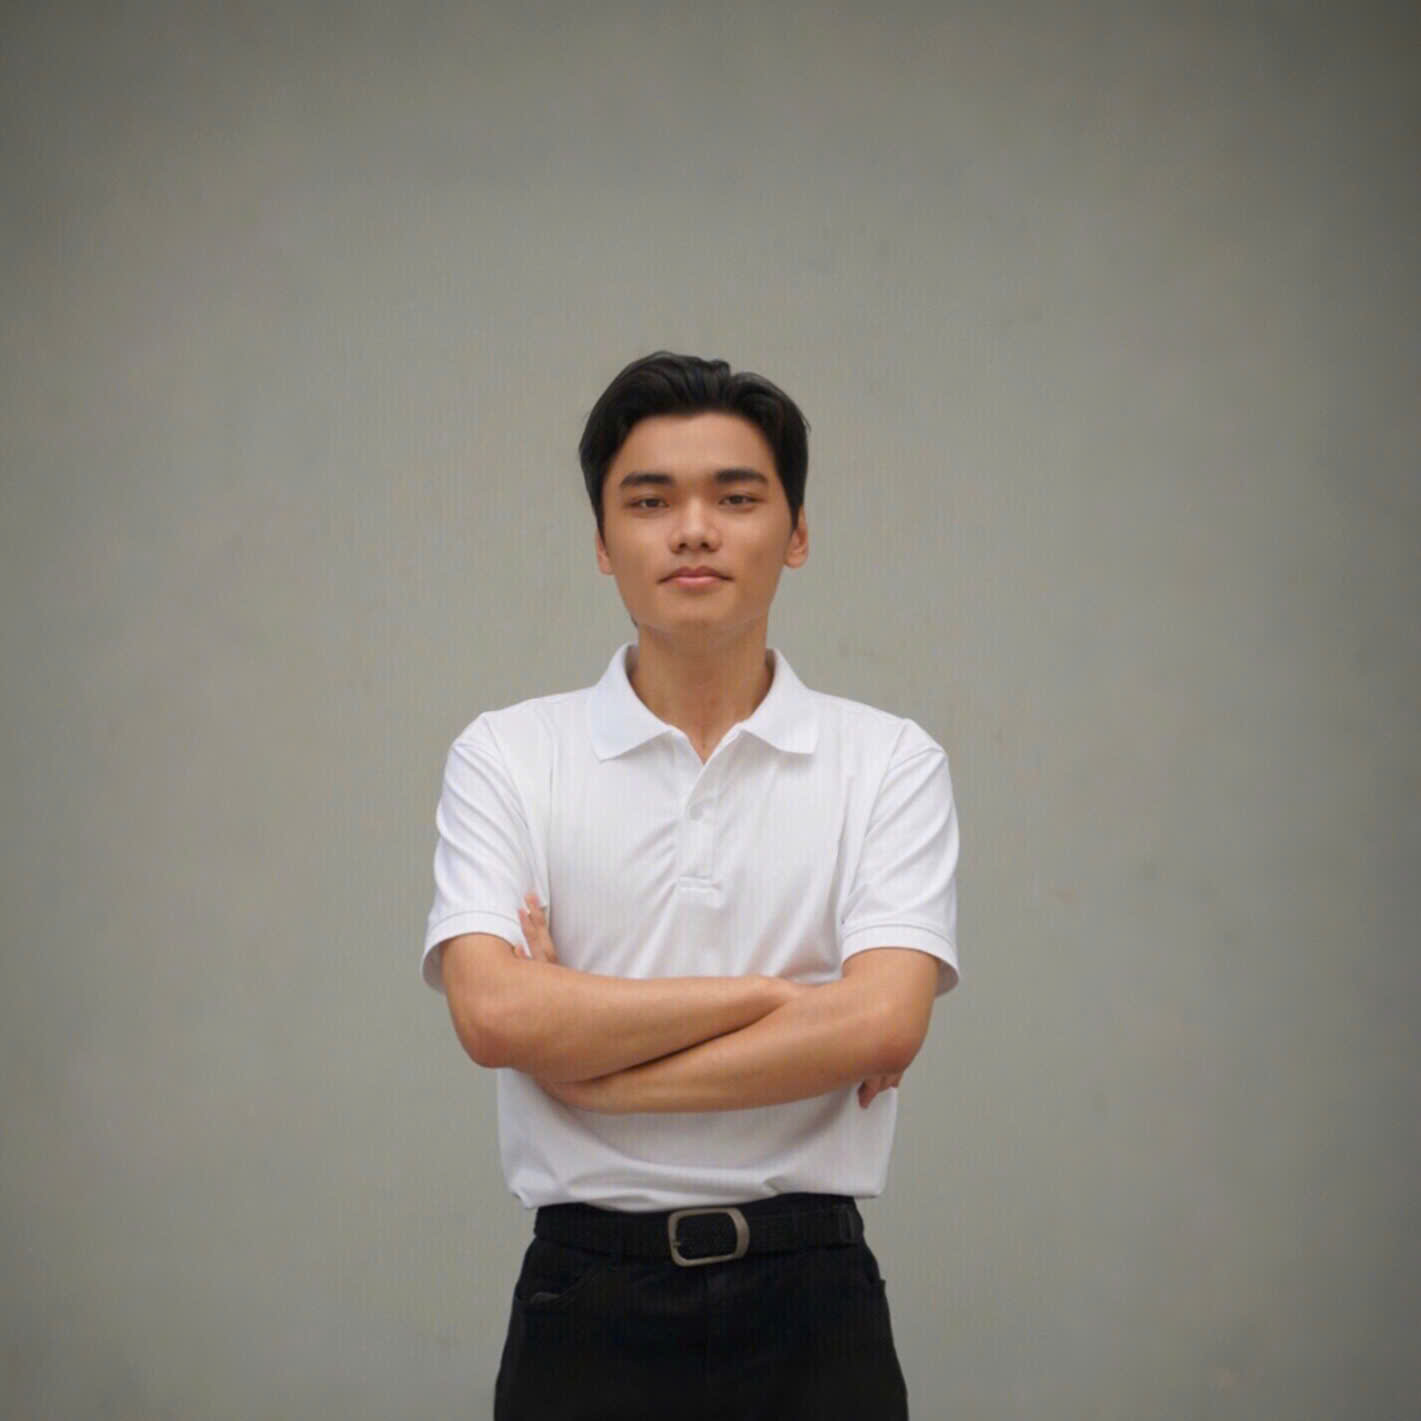
\includegraphics[width=3.2cm, trim={10cm 10cm 10cm 10cm }, clip]{../assets/avt.jpg} 
\end{minipage}
    \hspace{1cm}
\begin{minipage}[b]{0.75\textwidth}
    {\Huge\bfseries\color{primary} TRAN QUOC KHANG} \\ [7pt]
        \vspace{0.5cm}
    \small District 7, Ho Chi Minh City, Vietnam \\
    SĐT: 0987357707 \\
    Email: \href{mailto:trankhang2856@gmail.com}{trankhang2856@gmail.com} \\
    Linkedin: \href{https://linkedin.com/in/ryan-tr/}{linkedin.com/in/ryan-tr/}\\
    Github: \href{https://github.com/ryantr-statinops}{github.com/ryantr-statinops} \\
\end{minipage}

    \vspace{15pt}
% --- NỘI DUNG ---
\section{SUMMARY}
\begin{itemize}[leftmargin=*, noitemsep, topsep=0pt]
    \item Second-year student passionate about business, data science, technology and entrepreneurship.
    \item Focus areas: big data, data engineering, block chain, business development, tech startups.
    \item Building skills in data analysis, business analysis, and project management.
    \item Aiming to grow both soft skills and technical abilities for startup-oriented career.
\end{itemize}

\section{EDUCATION}
\noindent \textbf{Ton Duc Thang University} \hfill 2024 -- Present \\
\textit{Bachelor of Statistics (Field: Machine Learning and Quantitative Finance)} 
\vspace{8pt}
\begin{itemize}[leftmargin=*, noitemsep, topsep=0pt]
    \item \textbf{Applied Statistics \& Mathematical Economics:} Regression, Time Series, Multivariate Analysis, Econometrics. 
    \item \textbf{Core Focus:} Comprehensive training in Mathematical Statistics, Probability Theory, and Stochastic Processes.
    \item \textbf{Key Coursework:} Statistical Inference, Hypothesis Testing, Estimation Theory, and Advanced Data Analysis.
    \item \textbf{Technical Applications:} Extensive experience in statistical programming and modeling using \textbf{R}, Python, SQL, Excel, and Power BI to solve complex business and financial problems.
\end{itemize}

\section{WORK EXPERIENCE}
\noindent \textbf{HUB NETWORK HCMC} \hfill 04/2025 -- Present \\
\textit{HR Analyst} 
\begin{itemize}[leftmargin=*, noitemsep]
    \item Managing files and setting up automated tracking systems on Google Sheets using App Script.
    \item Analyzing participant data (300-400 customers) to identify target customer segments.
    \item Automating monthly HR reports to improve data accuracy.
\end{itemize}

\vspace{8pt}

\noindent \textbf{HUBLOCK - SMART DELIVERY LOCKER} \hfill 2024 -- Present \\
\textit{Business Development Executive} 
\begin{itemize}[leftmargin=*, noitemsep]
    \item Using Data Scraping techniques to collect potential B2B customer files.
    \item Building automated KPI trackers to monitor the progress of operations teams.
    \item Supporting connections with building managers to help achieve monthly contract targets.
\end{itemize}

\section{SKILLS}
\begin{itemize}[leftmargin=*, noitemsep]
    \item \textbf{Technical Skills:} Python, SQL, R, Power BI, Excel (Advanced), Google Apps Script.
    \item \textbf{Data Analysis:} Thu thập dữ liệu, Làm sạch dữ liệu, Phân tích thống kê, Trực quan hóa.
    \item \textbf{Soft Skills:} Giải quyết vấn đề, Tư duy phản biện, Làm việc nhóm, Thuyết trình.
\end{itemize}

\end{document}

